\documentclass{template/openetcs_article}
% Use the option "nocc" if the document is not licensed under Creative Commons
%\documentclass[nocc]{template/openetcs_article} 
\usepackage{lipsum,url}
\graphicspath{{./template/}{.}{./images/}}
\begin{document}
\frontmatter
\project{openETCS}

%Please do not change anything above this line
%============================
% The document metadata is defined below

%assign a report number here
\reportnum{OETCS/WP4/D4.1aV02}

%define your workpackage here
\wp{Work-Package 4: ``Verification and Validation''}

%set a title here
\title{Preliminary Evaluation Criteria on Verification and Validation}


%set a subtitle here
\subtitle{Version O2}

%set the date of the report here
\date{May 2013}

%define a list of authors and their affiliation here

\author{Hardi Hungar, Marc Behrens}

\affiliation{DLR\\
  Germany}
  
  
% define the coverart
\coverart[width=350pt]{chart}

%define the type of report
\reporttype{Description of work}


\begin{abstract}
%define an abstract here
  Evaluation criteria for tools and methods to be selected for use in
  V\&V activities are derived from a decription of their purpose
  (i.e., the activities to be performed with the help of the
  tools). This description is complemented by\\
    \texttt{WP41a-PreliminaryEvaluationCriteriaOnVAndVTables\_V02\_20130522.xml}. 
  
  \end{abstract}

%=============================
%Do not change the next three lines
\maketitle
\tableofcontents
\listoffiguresandtables
\newpage
%=============================

% The actual document starts below this line
%=============================


%Start here









%Examples are below


\section{Verification and Validation Activities}
\subsection{Definitions}

\paragraph{Verification}

Verification is an activity which has to be performed at each step of
the design. It has to be verified that the design step achieved its
goals. This consists at least of two parts:
\begin{itemize}
\item that the artifacts produced in the step are of the right type
  and contain allthe information they should. E.g., that the SSRS
  identifies all components addressed in SS~026, specifies their
  interfaces in sufficient detail and has allocated the functions to
  the components (this should just serve an example and is based on a
  guess what the SSRS should do)
\item that the artifact correctly implements the input requirements of
  the design step. These typically include the main output artifacts
  of the previous step. ``Correctly implements'' includes requirement
  coverage (tracing). This can and should be supported by some
  tools. Adequacy of such tools depends on things like format
  compatibility, degree of automation, functionality (e.g., ability to
  handle m-to-n relations). Depending on the design step (and the
  nature of the artifacts) different forms of verification will
  complement requirement coverage, with different levels of
  support. The step from SS~026 to the SSRS will mainly consist of
  manual activities besides things like coverage checks. Verifying a
  formal (executable) model against the SSRS can be supported by
  animation or simulation to e.g.\ execute test cases which have been
  designed to check compliance with the SSRS. Even formal proof tools
  may be employed to check or establish properties. Model-to-code steps
  offer far more options (and needs) for tool support. And tools or
  tool sets for unit test will support dynamic testing for requirement
  or code coverage. This may include test generation, test execution
  with report generation, test result evaluation and so on. Also, code
  generator verification (or qualification) may play a role,
  here. Integration steps mandate still other testing (or
  verification) techniques.
\end{itemize}
Summarizing, one may say that verification subsumes highly diverse
activities, and may be realized in very many different forms.

\paragraph{Validation}
%\nocite{*}
Validation is name for the activity by which the compliance of the end
result with the initial requirements is shown. In the case of
openETCS, this means that the demonstrator (or parts of it) are
checked against the SS~026 or one of its close descendants (i.e.,
SSRS). This will consist of testing the equipment according to a test
plan derived form the requirements and detailed into concrete test
cases at some later stage. Tool support for validation will thus
mainly concern test execution and evaluation, perhaps supplemented by
test derivation or test management. Ambitous techniques like formal
proof are most likely not applicable here.

Thus, the tool support for validation will not differ substantially
from that for similar verification activities.

One might also consider ``early'' validation activities, e.g.\
``validating'' an executable model against requirements from the
SS~026. These are not mandated by the standards and can per se not
replace design step verification. They may nevertheless be worthwhile
as means for early defect detection.

Further (mostly complementary) information on V\&V can be found in the
report on the CENELEC standards (D2.2).


\section{Evaluation Criteria}

\subsection{An Incomplete List of V\&V Activities}
\label{sec:table-verif-activ}

The following activities, which can all be performed or supported by
tools, might be relevant to openETCS. 
\begin{description}
\item[Tracing:] Relating requirement items to implementing items
\item[Animation:] Executing a model 
\item[Simulation:] code/model, perhaps with some environment representation 
\item[Formal proof of properties:] e.g.\ establishing some invariant
\item[Proof checking:] Verifying that a proof is correct (independently)
\item[Model checking:] Deciding properties of formal objects (specs,
  models, code)
\item[Test case generation:] From a formal object
\item[Test sequence generation:] Arranging test cases in a suitable way
\item[Test execution:] with subactivities test evaluation, report
  generation, perhaps test management, regression testing
\end{description}

Table~\ref{tab:techniques} lists some verification techniques which may be
used in openETCS to perform mandatory (according to the EN~50128)
verification steps. It is taken from the accompanying document\\
\texttt{WP41a-PreliminaryEvaluationCriteriaOnVAndVTables\_V02\_20130522.xml}. 
\\ The following abbreviations for design artifact are used in the table.
\begin{description}
\item[\texttt{C}:] code.
\item[\texttt{dM}:] A detailed model (from which code is derived or generated).
\item[\texttt{hM}:] A higher-level model (e.g., design specification model.
\item[\texttt{srsM}:] A model of the requirements (SRS).
\item[\texttt{SRS}:] The system requirements specification. 
\end{description}


\begin{table}[h]
\caption{Verification Steps and Techniques in openETCS} %title of the table
\label{tab:techniques}
% \begin{adjustbox}{width=\textwidth}
% \begin{tabular}{|l|p{0.2\textwidth}|p0.15\textwidth|c|c|c|c|p{0.2\textwidth}|p{0.2\textwidth}|}
% \hline
% \multicolumn{5}{|c|}{\textbf{T4.1 Identification of Tools and Profile Usage}} 
% \\\hline
% Verification Step & Description & Evaluation Category &
% \multicolumn{3}{|c|}appl.\ in verification step & validation& Verdict
% if passed & Verdict if not passed 
% \\&&&srsM$\rightarrow$SRS &dM$\rightarrow$hM &dM$\rightarrow$SRS &srsM$\rightarrow$SRS &
% \\\hline
% \end{tabular}
% \end{adjustbox}
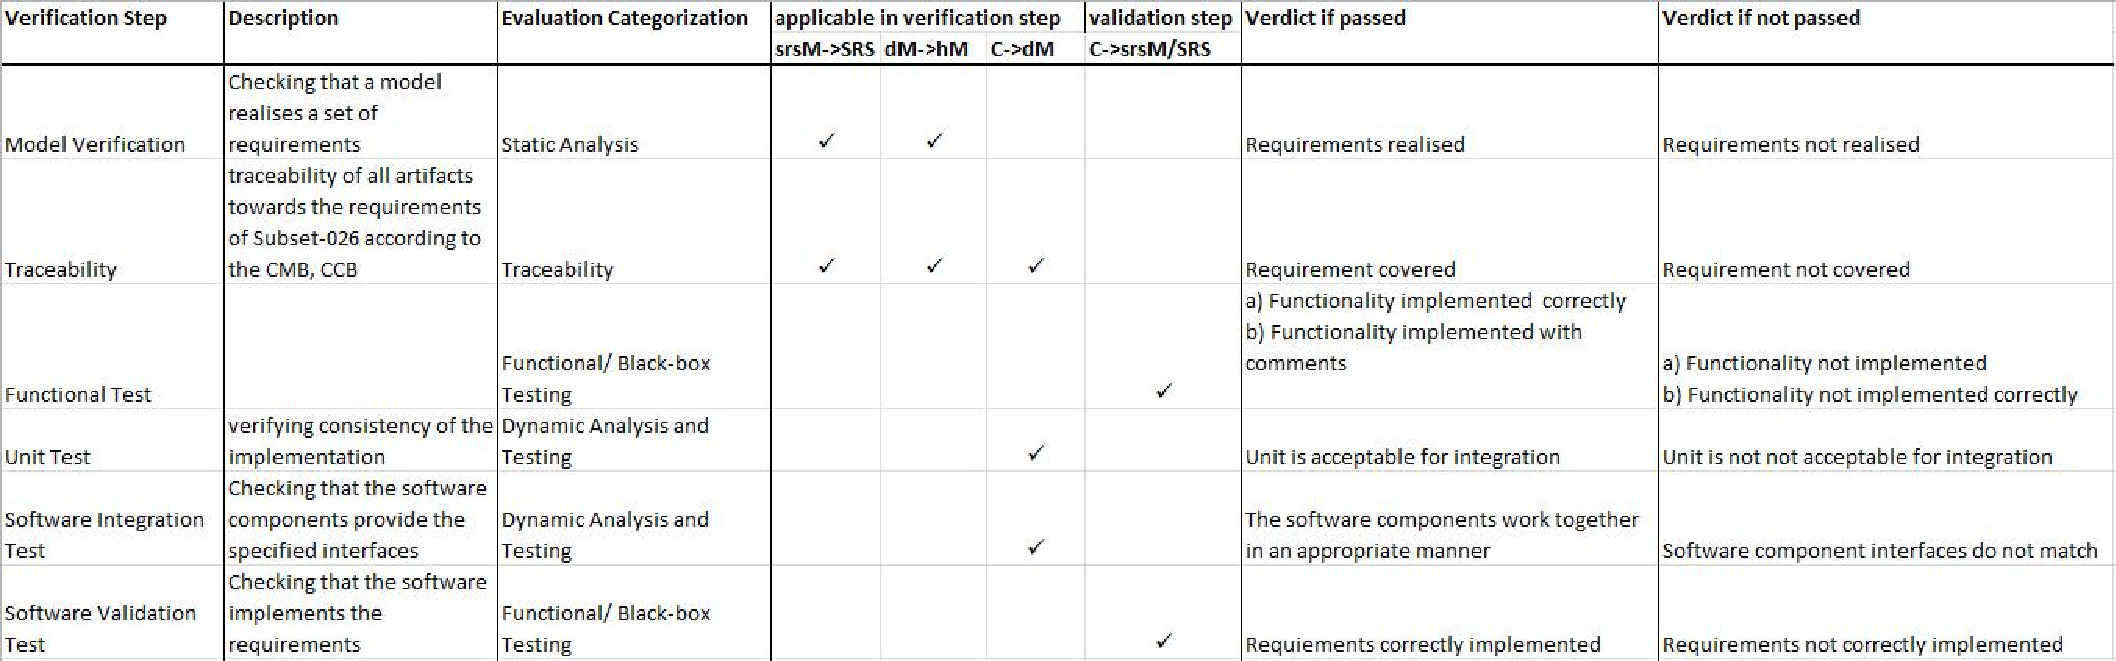
\includegraphics[width=\textwidth]{techniques.pdf}
\end{table}





\subsection{An Incomplete List of V\&V Tool Evaluation Criteria}
As broad as the range of V\&V activities and tools supporting them is
the set of evaluation criteria:

\begin{description}
\item[Effectiveness:] A tool must be able to perform a useful function
\item[Efficiency:] Very important for automatic routines like test
  case generation, model checking: They should not take forever or use
  infinite memory
\item[Vertical workflow integration:] input and output formats should
  match along a chain of dependent steps. Very specific input
  requirements can make a tool useless. More general, we should strive
  for a complete, rather well integrated tool chain
\item[Horizontal workflow integration:] Test management and test
  execution should go hand in hand.
\item[Qualifiabilty:] T2 or T3 qualification is required for some
  usages. Depends also on the process, as the failure of tool not
  being qualifiable in itself can be remedied by introducing a
  complemnting tool the checks the first's output (Example:
  Complementing code generation by verifying the equivalence of input
  and output)
\item[FLOSS:] of course (openETCS)
\end{description}

\section{Summary}
\label{sec:summary}

This document lists general criteria for the evaluation methods and
tools for verification and validation within openETCS. Detailing the
criteria needs more information on the design steps, which artifacts
are produced by them and by which methods. Concrete criteria are at
least as diverse as the different verification steps, and these depend
highly on the objects and how they are produced.

\bibliographystyle{unsrt}
%\bibliography{erdc}





%===================================================
%Do NOT change anything below this line

\end{document}
